\section{Лекция 20 (14.12)}

\subsection{Конечнообъёмное решение нестационарной задачи об обтекании кругового цилиндра}
TODO
\begin{figure}[h!]
\centering
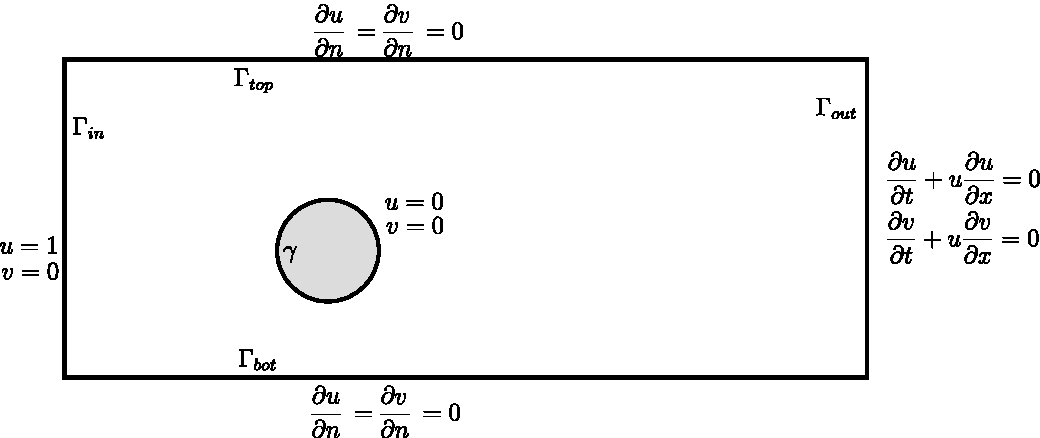
\includegraphics[width=0.8\linewidth]{cylinder_problem.pdf}
\caption{К постановке задачи об обтекании цилиндра}
\label{fig:cylinder-problem}

\end{figure}
\begin{equation}
\label{eq:ustar_fvm}
\left(1 + \frac{\tau}{\dt}\right) u^* + \tau \nabla\cdot(\vec u u^*) - \frac{\tau}{\Ren}\nabla^2 u^* = u + \frac{\tau}{\dt} \check u - \tau \dfr{p}{x}.
\end{equation}


\subsection{Задание для самостоятельной работы}
В тесте \ename{[cylinder2-fvm-pimple]} из файла \ename{cylinder_fvm_pimple_test.cpp}
приведено решение задачи об обтекании кругового цилиндра на неструктурированной конечнообъёмной сетке.
Нужно
\begin{enumerate}
\item
Визуализировать решение нестационарной задачи до момента $t = 100$,
\item
Продемонстировать эффект от поправки Rhie--Chow (см. аргумент \cvar{rhie_chow} в функции \cvar{compute_un_face})
на полях скорости и давления,
\item
Дополнить задачу уравнением для температуры вида \cref{eq:ns2d_nonstat_temperature}.
Использовать граничные условия(пользуясь обозначениями с \figref{fig:cylinder-problem}):
\begin{equation*}
\begin{aligned}
\Gamma_{in}:                &\quad T = 0,\\
\Gamma_{top}, \Gamma_{bot}: &\quad \dfr{T}{n} = 0, \\
\Gamma_{out}:               &\quad \dfr{T}{t} + u\dfr{T}{x} = 0,\\
\gamma:                     &\quad T = 1. \\
\end{aligned}
\end{equation*}
\item
Добавить процедуру вычисления интегрального числа Нуссельта $\Nun$ на временн\`{о}м слое.
\item
Провести расчёты для $\Ren=100$ и трёх чисел Пекле $\Pen = 30, 100, 1000$ до момента времени $t_{end} = 60$. Расчёты
проводить в релизной сборке.
\item
Сравнить полученные картины течения и графики $\Nun(t)$.
\end{enumerate}

\subsubsection{Уравнение для температуры}
После дискретизации по времени уравнения \cref{eq:ns2d_nonstat_temperature} с шагом $\dt$ оно примет вид
\begin{equation}
\label{eq:temperature_fvm}
\hat T + \dt \nabla\cdot(\vec u \hat T) - \frac{\dt}{\Pen}\nabla^2 \hat T = \check T,
\end{equation}
где $\hat T$ -- значение температуры на следующем временн\'{о}м слое.
Как видим, левая часть уравнения для температуры отличается от
левой части уравнения переноса для скорости \cref{eq:ustar_fvm} только множителями перед слагаемыми.
Типы граничных условий для этих уравнений также идентичны.
Значит матрицу левой части для уравнения температуры можно собирать по той же процедуре, что
и левую часть для $u^*$.
В тестовом рабочем классе эта процедура имеет сигнатуру
\begin{cppcode}
CsrMatrix CylinderFvmSimpleWorker::assemble_uv_lhs(double coef_u, double coef_conv, double coef_diff) const;
\end{cppcode}
где коэффициенты \cvar{coef_u}, \cvar{coef_conf}, \cvar{coef_diff} -- скалярные коэффициенты
перед слагаемыми свободным, конвективным и диффузным слагаемыми левой части.
Для сборки уравнения для $u^*$ эти коэффициенты равны 
$$
c_u = 1 + \frac{\tau}{\dt}, \quad c_{conv} = \tau, \quad c_{diff} = \frac{\tau}{\Ren}.
$$
Тогда для аппроксимации левой части уравнения для температуры нужно вызывать эту функцию
с коэффициентами
$$
c_u = 1, \quad c_{conv} = \dt, \quad c_{diff} = \frac{\dt}{\Pen}.
$$
Правая часть для внутренних точек коллокации будет аппроксимирована по стандартной конечнообъёмной процедуре:
\begin{equation*}
b^T_i = \arint{\check T}{E_i}{\vec x} = |E_i| \check T_i, \quad i = \overline{0, N_{cells}}.
\end{equation*}
Граничные условия для температуры содержат только одно неоднородное условие: $T=1$ на $\gamma$.
Поэтому для точек коллокации на границе $\gamma$ в правую часть следует поставить единицу
\begin{equation*}
b^T_i = 1, \quad i\in\gamma.
\end{equation*}

\subsubsection{Коэффициент теплоотдачи}
Из определния \cref{eq:integral_nu} интегральное число Нуссельта
расписывается как
\begin{equation}
\label{eq:fvm_nu}
\Nun = \arint{\dfr{T}{n}}{\gamma}{s}
= \sum_{s\in\gamma} \arint{\dfr{T}{n}}{\gamma_s}{s}
= \sum_{s\in\gamma}\left(\dfr{T}{n}\right)_{s} |\gamma_s|,
\end{equation}
где $s$ -- индексы всех граней, принадлежащих границе $s$,
а $\vec n$ -- нормаль к границе, внешняя к области расчёта.

\subsubsection{Порядок реализации}
\begin{enumerate}
\item
В рабочий класс необходимо добавить два новых поля: параметр $\Pen$ (\cvar{_Pe}) и массив $T$ (\cvar{_temperature}).
Параметр $\Pen$ необходимо пробросить в конструктор по аналогии с $\Ren$,
а массив $T$ инициализировать нулями внутри конструктора (длина массива равна количеству точек коллокации,
вычисляемой через метод \cvar{vec_size}).
\item
Для вычисления поля температуры добавить в рабочий класс новый метод
\begin{cppcode}
std::vector<double> CylinderFvmSimpleWorker::compute_temperature() const;
\end{cppcode}
который будет использовать текущую температуру \cvar{_temperature}
в качестве значения $\check T$ и возвращать новую температуру,
посчитанную по формуле \cref{eq:temperature_fvm}.
Этот метод будет иметь следующую реализацию
\begin{cppcode}
// 1. === Левая часть
CsrMatrix mat_temp = assemble_uv_lhs(1, _time_step, _time_step/_Pe);
// 2. === Правая часть
std::vector<double> rhs_temp(vec_size(), 0);
// 2.1 Внутренние точки коллокации
for (size_t icell=0; icell<_grid.n_cells(); ++icell){
	rhs_temp[icell] = _grid.cell_volume(icell) * _temperature[icell];
}
// 2.2 Граничные условия на цилиндре
for (size_t icolloc: _boundary_info.cyl){
	rhs_temp[icolloc] = 1;
}
// 2.3 Граничные условия на выходе
for (size_t icolloc: _boundary_info.output){
	rhs_temp[icolloc] = _temperature[icolloc];
}
// 3. === Решение СЛАУ
// 3.1 Массив с ответом.
//     Инициализируем текущей температурой в качестве первого приближения
std::vector<double> new_temperature(_temperature)
// 3.2 Вызываем решатель СЛАУ
AmgcMatrixSolver::solve_slae(mat_temp, rhs_temp, new_temperature);
// 4. === Возвращаем ответ
return new_temperature;
\end{cppcode}
\item
Вызывать этот метод следует в процедуре \cvar{to_next_time_step},
которая вызывается после окончания итераций на временн\`{о}м слое.
Возвращаемый процедурой массив нужно присвоить полю \cvar{_temperature},
тем самым обновив значение для температуры в классе.
\item
В процедуре \cvar{save_current_fields} добавить строчку
\begin{cppcode}
VtkUtils::add_cell_data(_temperature, "temperature", filepath, _grid.n_cells());
\end{cppcode}
для сохранения температуры в файл vtk.

\item
Добавить публичный метод \cvar{double CylinderFvmSimpleWorker::compute_nu() const}, который расчитывает
интегральный коэффициент теплоотдачи по текущему полю \cvar{_temperature}.
В реализации нужно запрограммировать формулу \cref{eq:fvm_nu}.
Необходимые методы для вычислений:
	\begin{itemize}
	\item
	Все индексы точек коллокации, лежащие на цилиндре
	\begin{cppcode}
	std::vector<size_t> cyl_collocs = _boundary_info.cyl;
	\end{cppcode}
	\item
	Индекс грани по индексу граничной точки коллокации \cvar{icolloc}
	\begin{cppcode}
	size_t iface = _collocations.face_index(icolloc);
	\end{cppcode}
	\item
	Производная температуры по нормали к грани с индексом \cvar{iface}
	\begin{cppcode}
	double dtdn = _dfdn_computer.compute(iface, _temperature);
	\end{cppcode}
	Поскольку в формуле \cref{eq:fvm_nu} используется не нормаль к грани,
	а внешняя нормаль к области, надо проверить, совпадают ли эти нормали.
	И если не совпадают (противонаправлены), то взять \cvar{dtdn} с обратным знаком:
	\begin{cppcode}
	if (_grid.tab_face_cell(iface)[0] == INVALID_INDEX){
		dtdn *= -1.0;
	}
	\end{cppcode}
	\item
	Для вычисления площади грани с индексом \cvar{iface}
	\begin{cppcode}
	double area = _grid.face_area(iface);
	\end{cppcode}
	\end{itemize}

\item
\clisting{open}{"test/cylinder_fvm_pimple_test.cpp"}
Вызывать этот метод нужно в цикле по времени в функции верхнего уровня
после обновления температурного поля:
\clisting{line}{"worker.to_next_time_step()"}
Например, для печати значения $\Nun$ в консоль следует написать
\begin{cppcode}
std::cout << "time=" << time << " Nu=" << worker.compute_nu() << std::endl;
\end{cppcode}
Можно осуществлять этот вызыв не на каждой временн\`{о}й итерации, а с некоторым заданным шагом.





\end{enumerate}
